\documentclass{jvfscript-de}
\usepackage{diff3style}
\usepackage{graphicx}
\graphicspath{ {./images/} }

%\usepackage{showframe}

\makeindex[title=Definitionen,intoc]

\renewcommand{\thechapter}{\S \arabic{chapter}}
\renewcommand{\thesection}{\arabic{chapter}.\arabic{section}}
\renewcommand{\thethm}{\arabic{chapter}.\arabic{thm}}

\begin{document}
	\frontmatter
	\maketitle
	
%	\setcounter{page}{1}
\tableofcontents
\newpage
%	\setcounter{page}{1}
\thispagestyle{plain}
Dieses Skript stellt keinen Ersatz für die Vorlesungsnotizen von Prof. Bahns dar und wird nicht nochmals von ihr durchgesehen, im Grunde sind das hier nur meine persönlichen Mitschriften. Beweise werde ich i.d.R. nicht übernehmen (weil das in \LaTeX{} einfach keinen Spaß macht). \hspace{\fill} glhf
\newpage
\mainmatter
\setstretch{1.15}			%Zeilenabstand. Kann man auch später nochmal reinhämmern, falls man es ändern will
	
	
	
	
	
	\chapter{Mannigfaltigkeiten}\lecture

\begin{defn}[Topologische Mannigfaltigkeit]\label{def1_1}\index{Mannigfaltigkeit}
	Eine \emph{$n$-dimensionale topologische Mannigfaltigkeit $M$} ist ein topologischer Hausdorff-Raum mit abzählbarer Basis der Topologie, der lokal euklidisch ist.
	\begin{itemize}
		\item lokal euklidisch:\\
			$ \foralll p \in M\ \existss U $ offene Umgebung von $p$, die homöomorph zu einer offenen Teilmenge des $\R^n$ ist, das heißt es gibt eine stetige, injektive Abbildung $ \varphi: U \to \R^n $ mit $ \varphi(U) $ offen in $\R^n$ (mit der Standardtopologie) und mit stetiger Umkehrfunktion $\varphi^{-1}: \varphi(U) \to M$.
			\image{1_1 homoeo}{12cm}
			\begin{rem*}
				$\varphi$ und auch $\varphi^{-1}$ sind offene Abbildungen, denn Bilder offener Mengen $ \tilde{U} \subset U $ (bezüglich $\varphi$), also $ \varphi(\tilde{U}) \subset \varphi(U) = \im(\varphi) $, sind Urbilder (bezüglich $\varphi^{-1}$) offener Mengen $\tilde{U}$ und somit offen (wegen der Stetigkeit von $\varphi^{-1}$)
				\image{1_1 offen}{8cm}
				Das heißt $U$ und $\varphi(U)$ sind als topologische Räume äquivalent (weil ihre offenen Mengen in $1-1$-Beziehung zueinander stehen).
			\end{rem*}
		\item Hausdorff-Raum:\\
			$ \foralll p \neq q \in M \ \existss U,V \subset M $ offen, sodass $ U \cap V = \emptyset,\ p \in U, q \in V $
			\image{1_1 hausdorff}{6cm}
			Erinnerung: In topologischen Räumen mit Hausdorff-Eigenschaft sind z.B. Grenzwerte von konvergenten Folgen eindeutig.
		\item Abzählbare Basis der Topologie:\\
			Es gibt ein höchstens abzählbares System $ \{U_1,U_2,U_3,\dots\} $ von offenen Mengen $ U_j \subset M $, sodass $ \foralll p \in M \ \forall $ Umgebungen $V$ von $p$ gibt es einen Index $j$, sodass $ p \in U_j \subset V $.
			\begin{rem*}
				Warum man dies fordert werden wir später bei der Existenz einer Teilung der Eins erkennen.
			\end{rem*}
	\end{itemize}
	\begin{notat*}
		Ist $M$ eine topologische Mannigfaltigkeit, $p \in M$, so nennt man einen Homöomorphismus $\varphi: U \to \tilde{U}$, $U$ offen in $M$, $\tilde{U} = \varphi(U)$ offen in $\R^n$, $p \in U$, eine \emph{(lokale) Karte} bei $p$. Gilt $ \varphi(p) = 0 $, sagt man, die Karte sei zentriert bei $p$.\\
		$U$ heißt \emph{Koordinatenbereich} von $\varphi$ und die Komponenten von $\varphi(q) = (x_1(q),\dots,x_n(q))$ (für $q \in U$) heißen \emph{lokale Koordinaten} von $q$.
		\begin{rem*}
			Ist $\varphi$ eine beliebige Karte bei $p$, so ist $\psi(q) = \varphi(q) - \varphi(p)$ eine bei $p$ zentrierte Karte.
		\end{rem*}
	\end{notat*}
	Ein System von Karten $ \set{(\varphi_\alpha,U_\alpha)}{\alpha \in A} $ heißt \emph{Atlas} von $M$, falls gilt $ M = \bigcup\limits_{\alpha \in A} U_\alpha $.
\end{defn}

\begin{exmp}
	\begin{enumerate}[label= {\roman*})]
		\item $M = \R^n$, versehen mit der Standardtopologie, denn $ \varphi: \R^n \to \R^n,\ \varphi(x) = x $ ist ein Homöomorphismus. $\R^n$ ist ein Hausdorff-Raum (vlg. Diff 2) und verfügt über eine abzählbare Basis: $ \set{\dot{B_r}(q) \ \text{offener Ball}}{r \in \Q, p \in \Q^n}. $
		\item Graphen von stetigen Funktionen:\\
			$ U \subset \R^n $ offen, $f: U \to \R^k$ stetig. Der \emph{Graph} $ \Gamma(f) = \set{(x,f(x))}{x \in U} \subset \R^n \times \R^k $, versehen mit der \emph{Teilraumtopologie}\footnote{
				Eine Teilmenge $M\subset \R^m$ ist mit der Teilraumtopologie versehen, falls $ U \subset M $ ist offen $ \iff \ \existss V \subset \R^m $ offen, sodass $ U = V \cap M $}
			ist eine $n$-dimensionale topologische Mannigfaltigkeit, denn $$ \varphi: \Gamma(f) \to \R^n, \varphi(x,y) = x,\ (x,y) \in \Gamma(f) \subset \R^n \times \R^k $$ bildet $\Gamma(f)$ homöomorph auf $U$ ab (die Umkehrfunktion ist die stetige Funktion $ \varphi^{-1}: U \to \R^n \times \R^k, \varphi^{-1}(x) = (x,f(x)) $). Die Hausdorff-Eigenschaft und die Abzählbarkeit einer Basis der Topologie übertragen sich direkt
			\begin{rem*}
				Wird nichts anders explizit gesagt, werden wir Teilräume stets als mit der Teilraumtopologie versehen ansehen.
			\end{rem*}
		\item Da (vgl. Diff2) jede Untermannigfaltigkeit $N$ sich lokal als Graph schreiben lässt und da die von uns betrachteten offenen Mengen in $N$ gerade die durch die Teilraumtopologie gegebenen sind folgt, dass eine Untermannigfaltigkeit im Sinne der Diff 2 eine topologische Mannigfaltigkeit im Sinne von \ref{def1_1} ist, explizit zum Beispiel:
		\item $\Sbb := \{ x \in \R^{n+1} \mid \|x\|_E = 1 \} $
			\image{1_2 sphere}{3cm}
			Wir konstruieren $2n+2$ Karten:\\
			Betrachte $ U_i^\pm = \{ x \in \R^{n+1} \mid x_i \gtrless 0 \} $. Sei $ \dot{\Bbb}^n = \{y \in \R^n \mid \|y\|_E < 1 \} $ und $ f: \dot{\Bbb}^n \to \R, f(y) = \sqrt{1-\|y\|_E^2}. $ Notiere für $ i = 1,\dotsc,n+1: x(\hat{i}) = (x_1,\dots, x_{i-1},x_{i+1},\dotsc,x_{n+1}) = (x_1,\dotsc,\hat{x_i},\dotsc,x_{n+1}) $.\\
			Es ist dann: $ U_i^\pm \cap \Sbb^n = \{ (x_1,\dotsc,x_{i-1}, \pm f(x(\hat{i})), x_{i+1},\dotsc,x_n \mid x(\hat{i}) \in \dot{\Bbb}^n \}, $ also nach Umsortieren gleich dem Graphen der Funktion $f$ beziehungsweise $-f$.\\
			Nach ii) sind also Karten durch
			\begin{gather*}
				\varphi_i^\pm : U_i^\pm \cap \Sbb^n \to \R^n,\ \varphi_i^\pm(U_i^\pm \cap \Sbb^n) = \dot{\Bbb}^n \\
				\varphi_i^\pm(x_1,\dotsc,x_{n+1}) = (x_1,\dotsc,\hat{x_i},\dotsc,x_{i+1} 
			\end{gather*} gegeben. Also ist $\Sbb^n$  eine $n$-dimensionale Mannigfaltigkeit. Wegen $\Sbb^n = \bigcup_{i=1}^{n+1} (U_i^+ \cap \Sbb^n \cup (U_i^- \cap \Sbb^n)$ liegt ein Atlas vor.
			\image{1_2 abbng}{12cm}
	\end{enumerate}
\end{exmp}



\begin{lem}\label{lem1_3}
	Sind $ M_1, \dotsc, M_k $ topologische Mannigfaltigkeiten mit Dimensionen $ n_1,\dotsc,n_k $, so ist das kartesische Produkt $ M_1 \times \dots \times M_k $ eine $ (n_1 + \dots + n_k) $-dimensionale topologische Mannigfaltigkeit.
\end{lem}

\begin{exmp*}
	Tori $ M = \underbrace{\Sbb^1 \times \dotsm \times \Sbb^1}_{k-\text{fach}} $ sind $k$-dimensionale Mannigfaltigkeiten, zum Beispiel $\Sbb^1 \times \Sbb^1$ eine 2-dimensionale:
	\image{1_3 exmp}{6cm}
\end{exmp*}

\begin{rem*}
	Die Hausdorff-Eigenschaft folgt nicht aus der lokalen Homöomorphie zu $\R^n$.
\end{rem*}
	
\begin{exmp*}
	$ M = (\R \setminus \{0\}) \times \{0\} \cup \{ (0,1)^T, (0,-1)^T \} \subset \R^2 $
	\image{1_3 counter1}{12cm}
	Wähle die Topologie auf $M$ so, dass $\varphi$ und $\psi$ homöomorph auf $\R$ abbilden. Dazu erklären wir die offenen Umgebungen von $ (0,\pm 1)^T $ als $ (I \setminus \{0\} \times \{0\}) \cup \{(0,\pm 1)\}$, wobei $I$ ein offenes Intervall um 0 ist. Sei dann $U$ eine offene Umgebung von $(0,1) $ und $\tilde{U}$ eine offene Umgebung von $(0,-1)$. Dann ist $U \cap \tilde{U} \neq \emptyset$ (da $I \setminus \{0\} \cap \tilde{I}\setminus\{0\} \neq \emptyset).$
	\image{1_3 counter2}{6cm}
\end{exmp*}

\begin{defn}[Kartenwechsel]\index{Mannigfaltigkeit!Kartenwechsel}
	Seien $ (\varphi_\alpha,U_\alpha), (\varphi_\beta,U_\beta) $ lokale Karten einer Mannigfaltigkeit $M$. Dann nennt man die Abbildung
	\[ \Phi_{\alpha\beta}: \varphi_\alpha(U_\alpha \cap U_\beta) \to \varphi_\beta(U_\alpha \cap U_\beta),\quad \Phi_{\alpha\beta} = \varphi_\beta \circ \varphi_\alpha^{-1} \]
	\image{1_4}{10cm}
	\emph{Kartenwechsel} (von $ \varphi_\alpha $ zu $\varphi_\beta$). Kartenwechsel sind also auf offene Teilmenge des $\R^n$ definierte Homöomorphismen.\\
	Ein Atlas heißt \emph{differenzierbar}, falls alle seine Kartenwechsel glatt, also $C^\infty$-Abbildungen, sind.
\end{defn}

\begin{rem*}
	In diesem Fall sind die Kartenwechsel Diffeomorphismen, das heißt auch die Umkehrabbildung ist wieder $C^\infty$, denn
	\[ \Phi_{\alpha\beta}^{-1} = \left(\varphi_\beta \circ \varphi_\alpha^{-1}\right)^{-1} = \varphi_\alpha \circ \varphi_\beta^{-1} = \Phi_{\beta\alpha} \]
	auf dem Definitionsbereich, wo die Abbildung definiert ist: $ \varphi_\beta(U_\alpha \cap U_\beta). $
\end{rem*}

\begin{defn}[Differenzierbare Struktur]\index{Mannigfaltigkeit!Differenzierbare Struktur}
	Sei $\Acal$ ein differenzierbarer Atlas (von $M$), dann bezeichnet man $\Dcal = \Dcal(\Acal)$ die Menge \emph{aller} Karten von $M$, die mit allen Karten aus $\Acal$ glatte Kartenwechsel haben,
	\[ \Dcal(\Acal) = \set{(\psi,U) \ \text{Karten}}{\bound{\psi \circ \varphi^{-1}}{\varphi(V \cap U)}, \bound{\varphi \circ \psi^{-1}}{\varphi(V \cap U)} \in C^\infty \ \text{für alle } (\varphi,V) \in \Acal}. \]
	\begin{rem*}
		$\Dcal(\Acal)$ ist \emph{maximal} in dem Sinn, dass es keine weiteren Karten gibt, die $C^\infty$-Kartenwechsel mit den Karten aus $\Acal$ hätten, die nicht schon in $\Dcal(\Acal)$ liegen. $\Dcal(\Acal)$ ist also der größte differenzierbare Atlas, der $\Acal$ enthält.
	\end{rem*}
	\begin{notat*}
		Ein maximaler, differenzierbarer Atlas auf einer Mannigfaltigkeit $M$ heißt \emph{differenzierbare Struktur} (auf $M$). Eine Mannigfaltigkeit zusammen mit einer differenzierbaren Struktur heißt \emph{differenzierbare Mannigfaltigkeit}.
	\end{notat*}
\end{defn}

\begin{rem*}
	\begin{enumerate}[label = {\roman*})]
		\item Es genügt, einen möglichst kleinen Atlas anzugeben, da dieser die differenzierbare Struktur festlegt.
		\item ACHTUNG: Zwei Atlanten $ \Acal_1,\Acal_2 $ einer Mannigfaltigkeit $M$ führen nur dann zur selben differenzierbaren Struktur, wenn für alle $ (\varphi,U) \in \Acal_1 $ und $ (\psi,V) \in \Acal_2 $ die Kartenwechsel glatt sind.
	\end{enumerate}
\end{rem*}

\begin{exmp*}
	$ \Sbb^n $ mit den oben eingeführten Karten ist eine glatte Mannigfaltigkeit.
\end{exmp*}
	

	\addtocounter{thm}{1}\lecture
\begin{defn}[Differenzierbare Abbildung zwischen Mannigfaltigkeiten]\index{Mannigfaltigkeit!Differenzierbare Abbildung zwischen Mannigfaltigkeiten}
	Seien $M,N$ differenzierbare Mannigfaltigkeiten, $M$ $m$-dimensional, $N\ n$-dimensional. Sei $ f: M \to N $  stetig. $f$ heißt \emph{(stetig) differenzierbar/glatt} im Punkt $p \in M$, falls für eine (und damit für jede!) Karte $ (\varphi,U) $ bei $p$ und eine (und damit für jede) Karte $ (\psi,V) $ bei $f(p)$ gilt
	\[ \psi \circ f \circ \varphi^{-1}: \varphi \left( f^{-1}(V) \cap U \right) \to \R^n \]
	ist (stetig) differenzierbar/glatt in $\varphi(p).$
	\image{1_7}{14cm}
\end{defn}

Diese Eigenschaft ist tatsächlich unabhängig von der Wahl der Karten $\varphi$ und $\psi$: Seien $ \varphi' $ und $\psi'$ weitere Karten bei $p$ beziehungsweise $f(p)$, dann ist 
\[ \psi \circ f \circ \varphi^{-1} = \psi' \circ \left( \psi'^{-1} \circ \psi \right) \circ f \circ \left( \varphi^{-1} \circ \varphi' \right) \circ \varphi'^{-1} \]
genau dann (stetig) differenzierbar/glatt in $p$, wenn $\psi' \circ f \circ \varphi'^{-1}$ (stetig) differenzierbar/glatt in $p$ ist, denn die Kartenwechsel $\psi'^{-1} \circ \psi, \varphi^{-1} \circ \varphi'$ sind glatt.

\begin{rem*}
	$ C^\infty (M,N) := \{ f: M \to N \ \text{glatt}\} $\\
	Die differenzierbaren Mannigfaltigkeiten mit $C^\infty$-Abbildungen bilden eine Kategorie, die unter Verknüpfungen abgeschlossen ist, das heißt $ f, g \in C^\infty \implies f \circ g \in C^\infty. $
\end{rem*}

\begin{defn}[Diffeomorphismus]\index{Diffeomorphismus}
	Eine Abbildung $ f: M \to N $ nennt man \emph{Diffeomorphismus}, falls $ f \in C^\infty $ umkehrbar ist mit $ f(M)=N $ und die Umkehrfunktion wieder $C^\infty$ ist. Gibt es einen Diffeomorphismus $ M \to N $ (somit auch einen Diffeomorphismus $N \to M$) nennt man $M$ und $N$ diffeomorph, $M \cong N$.
\end{defn}

\begin{rem}
	\begin{enumerate}[label = {\roman*})]
		\item Aufgabe 3 Blatt 1: Verschiedene differenzierbare Strukturen auf $\R$: Atlanten $ \{\id_\R\}, \{\varphi: x \mapsto x^3\} $, aber $ (\R,\{\id_\R\}) \overset{\cong}{\longrightarrow} (\R,\{\varphi\}) $ diffeomorph.\\
			Allgemeiner: $ U \subset \R^n $ offen, Atlas $ \Acal = \{\id_U\} \rightarrow $ "Standard-Differenzierbare-Struktur". Jeder Homöomorphismus $ \varphi:  U \to V \in \R^n $ gibt auch einen Atlas und eine differenzierbare Struktur. Sie ist genau dann die Standard differenzierbare Struktur, wenn $\varphi$ als Abbildung $ U \subset \R^n \to \tilde{U} \subset \R^n $ ein Diffeomorphismus ist.\\
			ACHTUNG! Als differenzierbare Mannigfaltigkeiten sind $ (U,\{\id_U\}) $ und $(U,\{\varphi\})$ aber auch dann diffeomorph, wenn $\varphi: U \to \tilde{U}$ kein Diffeomorphismus ist! Denn $ \varphi: (U,\{\varphi\}) \to (U,\{\id_U\}) $ ist ein Diffeomorphismus differenzierbarer Mannigfaltigkeiten: $ \id_U \circ \varphi \circ \varphi^{-1} = \id_U $ ist ein Diffeomorphismus $ U \to U $.
		\item Sehr viele Sätze befassen sich damit, ob es auf einer Mannigfaltigkeit verschiedene differenzierbare Strukturen gibt, sodass die entstehenden differenzierbaren Mannigfaltigkeiten nicht diffeomorph sind. Auf $ \Sbb^7 $ gibt es genau 15 verschiedene differenzierbare Strukturen, die nicht diffeomorph zueinander sind (Milnor + Kervaire 1963, "exotische Sphären", erstes Beispiel Milnor 1956).
		\item Unser Thema hier: Strukturen, die unter der Anwendung von Diffeomorphismen invariant sind. Daher können wir lokale Eigenschaften immer auf offenen Mengen im $\R^n$ untersuchen (also mit Hilfe von Karten und Koordinaten). Das heißt konkret: Statt $ f : U \subset M \to N $ zu betrachten mit $M$ und $N$ als differenzierbare Mannigfaltigkeiten betrachten wir $ \psi \circ f \circ \varphi^{-1} $ mit $ (\varphi,\tilde{U}), \tilde{U} \subset U, $ Karte von $M$ und $ (\psi,V) $ Karte von $N$ mit $ f(\tilde{U})\subset V $, also eine Abbildung von einer offenen Menge $\subset \R^m$ in eine offene Menge $\subset \R^n$.
		\item Es ist keine Einschränkung, Glattheit der Kartenwechsel zu fordern. Denn es gilt: Ist $\Acal$ ein Atlas von $M$ mit $C^1$-Kartenwechseln, so gibt es zu jedem $l,\ 1 \leq l \leq \infty,$ einen Atlas $ \tilde{\Acal} $ von $M$, sodass die Kartenwechsel von $\tilde{\Acal}$ $C^l$-Abbildungen sind und so, dass die Kartenwechsel von $\tilde{\Acal} \cup \Acal$ $C^1$ sind [Whitney, 1936], das heißt für $l = \infty$ ist $ (M,\Dcal(\tilde{\Acal})) $ eine differenzierbare Mannigfaltigkeit im Sinne unserer Definitionen.
		\item Es gibt topologische Mannigfaltigkeiten, die keinen Atlas besitzen, der $C^1$-Kartenwechsel hat (somit auch keine differenzierbare Struktur in unserem Sinn).
	\end{enumerate}
\end{rem}

\section{Untermannigfaltigkeiten}

\begin{defn}[Topologische Untermannigfaltigkeit]\index{Mannigfaltigkeit!Untermannigfaltigkeit}\index{Mannigfaltigkeit!glatte Einbettung}
	$ N \subset M, \dim(M) = n+k, $ heißt \emph{$n$-dimensionale (topologische) Untermannigfaltigkeit} der (topologischen) Mannigfaltigkeit $M$, falls es zu jedem Punkt $p \in N$ eine Karte $ (\varphi,U)$ von $M$ bei $p$, $ \varphi: U \to \R^n \times \R^k $, gibt, sodass $ \varphi(U \cap N) = \varphi(U) \cap (\R^n \times \{0\}). $ Eine Karte von $M$ mit dieser Eigenschaft heißt \emph{$N$ angepasst}.\\
	Ist $M$ differenzierbar, so heißt $N$ \emph{differenzierbare Untermannigfaltigkeit} von $M$, falls es zu jedem $p \in N$ angepasste Karten aus der differenzierbaren Struktur von $M$ gibt. Die Gesamtheit der Karten 
	$$ \big\{ \varphi: U \cap N \to \varphi(U) \cap \vertarrowbox[1ex]{\R^n}{$ \R^n \cong \R^n \times \{0\} $} \mid \varphi\ \text{angepasste Karte aus der diff'baren Struktur von } M \big\} $$
	ist ein differenzierbarer Atlas für $N$.
	\image{1_10}{12cm}
	\begin{exmp*}
		$ \Sbb^n $ ist eine Untermannigfaltigkeit des $\R^{n+1}$. Angepasste Karten:
		\[ \psi_{\pm i}: U_i^\pm \to \R^{n+1},\ \psi_{\pm i}(x) = \left( x \left( \hat{i} \right),x_i \right) \]
	\end{exmp*}
	Man nennt eine glatte Abbildung $ f: \tilde{M} \to M $ eine \emph{glatte Einbettung}, falls $ f\left( \tilde{M} \right) \subset M $ eine differenzierbare Untermannigfaltigkeit von $M$ ist und $ f: \tilde{M} \to f\left( \tilde{M} \right) $ ein Diffeomorphismus.
\end{defn}

\begin{thm}
	Sei $M$ eine $(n+k)$-dimensionale differenzierbare Mannigfaltigkeit, $ N \subset M$ eine Teilmenge. Dann ist $N$ eine $n$-dimensionale differenzierbare Untermannigfaltigkeit $ \iff \ \foralll p \in N \ \exists $ Umgebung $U$ von $p$ in $M$ und eine glatte Abbildung $ f: U \to \R^k$, mit $ Df(q) $ von maximalem Rang $k\ \foralll q \in U$, sodass $ U \cap N = f^{-1}(0). $
\end{thm}

\begin{exmp*}
	Betrachte den Torus $ \pi = \Sbb^1 \times \Sbb^1 $. Diese Mannigfaltigkeit lässt sich als differenzierbare Untermannigfaltigkeit des $\R^3$ realisieren: Sei $ 0 < r < R $. Rotiere den Kreis von Radius $r$ um $ (R,0) $ in der $(x,z)$-Ebene um die $z$-Achse, so entsteht eine zu $ \Sbb^1 \times \Sbb^1 $ diffeomorphe Untermannigfaltigkeit. Dazu zunächst folgende Beobachtung:
	\addtocounter{thm}{1}
	\begin{rem}
		Differenzierbare Struktur auf Produkt-Mannigfaltigkeiten:\\
		Die Kartenwechsel der Karten aus Lemma \ref{lem1_3} 
		\[ \varphi_1 \times \dotsm \times \varphi_k: \underset{\subset M_1}{U_1} \times \dotsm \times \underset{\subset M_k}{U_k} \to \R^{n_1} \times \dotsm \times \R^{n_k} \]
		sind glatt, wenn die $M_j$ differenzierbare Mannigfaltigkeiten sind, denn 
		\[ \psi_1 \dotsm \psi_k \circ (\varphi_1 \times \dotsm \times \varphi_k)^{-1} = \psi_1 \circ \varphi_1^{-1} \times \dotsm \psi_k \circ \varphi_k^{-1}. \]
	\end{rem}
	Die Tori $ \Sbb^1 \times \dotsm \times \Sbb^1 $ sind somit (kanonisch) mit einer differenzierbaren Struktur versehen. Die Homöomorphie von $\pi$ mit der Rotationsfläche ist tatsächlich ein Diffeomorphismus.
\end{exmp*}

\begin{rem*}
	Bisher haben wir topologische Mannigfaltigkeiten betrachtet und diese dann mit einer differenzierbaren Struktur versehen.\\
	Gegeben eine Familie von Karten, die gewisse Eigenschaften haben, kann man direkt eine Topologie und eine differenzierbare Struktur auf einer Mannigfaltigkeit in einem Schritt definieren, wie das folgende Lemma zeigt:
\end{rem*}

\begin{lem}\label{1.14}
	Sei $M$ eine Menge und $ \{\varphi_\alpha: U_\alpha \to \R^n \mid \alpha \in A\}, U_\alpha \subset M, $ eine Familie von Abbildungen mit folgenden Eigenschaften:
	\begin{enumerate}[label={\roman*})]
		\item Es gibt eine abzählbare Menge $ I \subset A $, sodass $ M = \bigcup\limits_{\alpha \in I}U_\alpha. $
		\item Für $ p,q \in M, p \neq q, $ gibt es ein $ U_\alpha $, sodass $ p,q \in U_\alpha $ oder es gibt $ U_\alpha,U_\beta, U_\alpha \cap U_\beta = \emptyset, $ mit $ p \in U_\alpha, q \in U_\beta. $
		\item Für jedes $ \alpha \in A $ ist $ \varphi_\alpha $ eine Bijektion von $ U\alpha $ auf eine \emph{offene} Teilmenge $ \varphi_\alpha(U_\alpha) \subset \R^n $.
		\item Für alle $ \alpha,\beta \in A $ sind $ \varphi_\alpha(U_\alpha \cap U_\beta) $ und $ \varphi_\beta(U_\alpha \cap U_\beta) $ offen in $\R^n$.
		\item Für alle $ \alpha,\beta \in A $ ist die Abbildung $ \varphi_\beta \circ \varphi_\alpha^{-1}: \varphi_\alpha( \underset{\subset \R^n}{U_\alpha \cap U_\beta} ) \to \varphi_\beta( \underset{\subset \R^n}{U_\alpha \cap U_\beta} ) $ glatt.
	\end{enumerate}
	Dann ist $M$ eine differenzierbare Mannigfaltigkeit, deren differenzierbare Struktur eindeutig durch die Forderung festgelegt ist, dass die $ (\varphi_\alpha,U_\alpha) $ glatte Karten sind, das heißt dass alle Kartenwechsel glatt sind.
\end{lem}
	\chapter{Der Tangentialraum}\lecture

Erinnerung (Diff 2): Sei $ M \subset \R^n $ eine Untermannigfaltigkeit, $p \in M$. Ein Tangentialvektor $v \in \R^n$ an $M$ in $p$ ist von der Form $ v = \gamma'(0) $, wobei $ \gamma: (-\epsilon,\epsilon) \to M $ mit $\gamma(0) = p$ eine in $M$ verlaufende $C^1$-Kurve ist. Der \emph{Tangentialraum} $T_pM$ (an $M$ in $p$) ist die Menge aller Tangentialvektoren. 
\begin{itemize}
	\item Ist $ U \subset \R^n $ offen, $p \in U$, $f: U \to \R^{n-m}$ $C^1$ mit $ M \cap U = \{x \in U \mid f(x) = 0\} $ und $rang(Df(p)) = n-m.$ Dann ist der Tangentialraum in $p$ an $M$ $ T_pM = \ker(Df(p)) \subset \R^n $ ($m$-dim. Unterraum).
	\item Ist $ \psi: V \to \R^n $ eine lokale Parametrisierung von $M$ bei $p$, so sind $ \del{j}\psi,\ d=1,\dotsc,m$, Basisvektoren $ V \subset \R^n $ für $ T_pM $.
\end{itemize}

\begin{exmp*}
	$ \Sbb^2 \subset \R^3,\ T_pM = p^\bot $, denn $ f: \R^n \to \R, f(x) = 1-\|x\|^2 $ für $ p \in \Sbb^2 $, sodass $p_i > 0$ oder $<0$ beschreibt $ \Sbb^2 \cap U_i \ni p, U_i = \{x \in \R^3 \mid x_i > 0 $ oder $ < 0\} $ als Nullstellengebilde und $ Df(p) = -2p. $
	\incfig{2}{14cm}
\end{exmp*}

Zur Verallgemeinerung auf Mannigfaltigkeiten\footnote{von nun an betrachten wir nur noch differenzierbare Mannigfaltigkeiten} überlegen wir zunächst, dass 2 Kurven zum selben Tangentialvektor führen, wenn sie in einer Umgebung von $p$ Übereinstimmen. Formalisiert und verallgemeinert führen wir daher ein:

\begin{defn}[Keime]\index{Keime}
	Auf $ \{f \mid f: U \to N,\ U $ offene Umgebung von $p \in M\} $ definiert 
	$$ f \sim g \iff \existss \text{offene Umgebung } V \ \text{von } p \text{, sodass } \bound{f}{V} = \bound{g}{V} $$
	eine Äquivalenzrelation. Eine Äquivalenzklasse bezüglich $\sim$ nennt man \emph{Keim} einer Abbildung $M \to N$ bei $p$. Ist $ f $ $C^1$/glatt bei $p$, so auch alle Elemente der von $f$ repräsentierten Klasse $\bar{f}$. Man spricht in dem Fall von $C^1$/glatten Keimen. Wir schreiben $ \Ecal^1(p) $ bzw. $\Ecal^\infty(p)$ für die Menge aller $C^1$ bzw. glatten Keime bei $p \in M$ mit Werten in $\R$ ("Funktionskeime") $ (M,p) \to \R $.
\end{defn}

\begin{rem}
	\begin{enumerate}[label={\roman*})]
		\item $\Ecal^1(p)$ und $\Ecal^\infty(p)$ bilden eine Algebra (denn die Bildung von Äquivalenzklassen ist mit der punktweisen Addition und Multiplikation verträglich).
		\item Ist $ \bar{f}: (M,p)\to N $ ein $C^1$/glatter Keim bei $p \in M$, so definiert er einen Homomorphismus von Algebren \big($\Ecal(f(p))$ Keime $(N,f(p)) \to \R$\big)
		\[ f^*: \Ecal^{1/\infty} (f(p)) \to \Ecal^{1/\infty} (p) \ \text{vermöge } f^* \big( \bar{h} \big) = \bar{h} \circ \bar{f} \quad \text{"pullback", "Zurückziehung"} \]
		Offensichtlich ist das unabhängig von der Wahl des Repräsentanten.
		\incfig{2_2}{14cm}
		Es gilt $\id^* = \id$ und $(f \circ g)^* = g^* \circ f^*$. Insbesondere induziert ein bezüglich Komposition invertierbarer Keim $\bar{f}$ ($ \bar{f} \circ \bar{f}^{-1} = \bar{f} \circ \overbar{f^{-1}} = \id $) einen Isomorphismus $f^*, f^{-1 *} \circ f^* = \id$.
		\item Spezialfall: Ist $\varphi$ eine um $p \in M$ zentrierte Karte, so definiert $\varphi$ einen invertierbaren Keim $ \overbar{\varphi}: (M,p) \to \R^n $ mit $\varphi(p)=0$ und somit einen Isomorphismus $ \varphi^*: \Ecal^{1/\infty}_n \to \Ecal^{1/\infty} (p) $, wobei $ \Ecal_n = \{$Funktionskeime bei $0 \}, $ das heißt man kann sich auf Keime aus $\Ecal_n$ beschränken.
	\end{enumerate}
\end{rem}

\section{3 Definitionen des Tangentialraums}

\begin{defn}[algebraische Definition]\index{Tangentialraum}\index{Derivation}
	Eine \emph{Derivation} von $\Ecal^\infty(p)$ ist eine lineare Abbildung $X: \Ecal^\infty(p) \to \R$, die der folgenden Leibniz-Regel genügt:
	\[ X(\bar{f} \cdot \bar{g}) = X(\bar{f}) \cdot g(p) + f(p) \cdot X(\bar{g}). \]
	Der \emph{Tangentialraum} $T_pM$ in $p$ ist der Vektorraum der Derivationen von $\Ecal^\infty(p)$.\\
	Ein glatter Keim $ \bar{f}: (M,p) \to N $ induziert einen Algebra-Homomorphismus $ f^*: \Ecal^\infty (f(p)) \to \Ecal^\infty (p) $ und somit eine (lineare) Abbildung, die \emph{Tangentialabbildung} (oder Differential) $ T_pf: T_pM \to T_{f(p)}N, X \mapsto X \circ f^*. $
\end{defn}

\begin{rem*}
	\begin{enumerate}[label={\roman*})]
		\item Es gilt 
		$$ T_p \big( \bar{g} \circ \bar{f} \big) = T_{f(p)} \bar{g} \circ T_p\bar{f}\quad \foralll \bar{f}: (M,p) \to N, \bar{g}: (N,f(p)) \to \tilde{N} \in C^\infty, $$
		denn für $\bar{h} \in \Ecal^\infty (g(f(p)))$ gilt
		\begin{align*}
			X \circ \Big( \big( \bar{g} \circ \bar{f} \big)^* \Big) \big( \bar{h} \big) &= X \big( \bar{h} \circ \big( \bar{g} \circ \bar{f} \big) \big)\\
			&= \big( X \circ f^* \big) \big( \bar{h} \circ \bar{g} \big)\\
			&= T_{f(p)}\bar{g} \big( X \circ f^* \big)(h)\\
			\text{und } \big( T_{f(p)} \bar{g} \circ T_p\bar{f} \big) &= T_{f(p)}\bar{g} \big( X \circ \bar{f}^* \big)\big( \bar{h} \big)
		\end{align*}
		\item Ist $\bar{\varphi}: (M,p) \to \R^n$ ein Keim einer bei $p$ zentrierten Karte, so ist $ \Ecal_n^\infty \overset{\cong}{\underset{\varphi^*}{\longrightarrow}} \Ecal^\infty(p) $ isomorph und $ T_pM \overset{\cong}{\underset{T_p \varphi}{\longrightarrow}} T_0\R^n $. 
	\end{enumerate}
\end{rem*}

$T_0\R^n$ hat eine besonders einfache Beschreibung:

\begin{lem}
	Die partiellen Ableitungen $ \del{j} $ in 0 bilden eine Basis von $ T_0\R^n. $
\end{lem}

\begin{rem*}
	$ \bound{\del{j}}{0} \overset{1:1}{\longleftrightarrow} e_j \in \R^n. $ Somit ist $ T_0\R^n \cong \R^n $ als Vektorraum.
\end{rem*}

\begin{thm}
	Seien $ (x_1,\dotsc,x_m),(y_1,\dotsc,y_n) $ lokale Koordinaten bei $p \in M, q \in N$, gegeben durch bei $p$ bzw. $q$ zentrierte Karten $ \varphi,\psi $ (das heißt $ x_i(\tilde{p}) = \varphi_i (\tilde{p}) $ mit $(\varphi,U)$ lokale Karte bei $p \in M, \tilde{p} \in U, \varphi(p) = 0$. Analog für $y_j$.)\\
	Dann sind $ \Big\{ \bound{\frac{\del{}}{\del{x_1}}}{0}, \dotsc, \bound{\frac{\del{}}{\del{x_m}}}{0} \Big\} $ bzw. $ \Big\{ \bound{\frac{\del{}}{\del{y_1}}}{0}, \dotsc, \bound{\frac{\del{}}{\del{y_n}}}{0} \Big\} $ Basen von $ T_0\R^m \cong T_pM $ bzw. $ T_0\R^n \cong T_qN $.\\
	Die Tangentialabbildung eines $C^\infty$-Keimes $\bar{f}: (M,p) \to N$ ist bezüglich dieser Basen durch die Jacobimatrix $ D( \vertarrowbox[1ex]{\psi \circ f \circ \varphi^{-1}}{Keim $ (\R^m,0) \to \R^n $} ) (0): \R^m \to \R^n $ gegeben.
	\[ \begin{tikzcd}
		T_pM \arrow{r}{Df} \arrow{d}{\varphi} & T_{f(p)}N \arrow{d}{\psi}\\
		T_0\R^m \arrow[r] & T_0\R^n
	\end{tikzcd} \]
\end{thm}

\begin{rem*}	
	Hierbei setzen wir $ \varphi^{-1} $ außerhalb von $ \varphi(U) $ glatt auf $\R^m$ fort.
\end{rem*}

\begin{exmp*}
	\begin{minipage}{\linewidth}
		\begin{wrapfigure}{R}{0.3\textwidth}
			\wrapincfig{2_5_1}{0.1\textwidth}
		\end{wrapfigure}
		$ M = \Sbb^1, p = (0,1,0)^T, \begin{aligned}[t]
			&\varphi: U_2^+ \cap \Sbb^2 \to \R^2, \\&\varphi(x) = (x_1,x_3)
		\end{aligned} $
	\end{minipage}
		
		Basis des Tangentialraums $ T_0\R^2 $ $ \bound{\del{1}}{0},\bound{\del{2}}{0} $\\
		$ f_{1,2}: \Sbb^2 \to \Sbb^2, \begin{aligned}[t]
			&f_1(x) = (x_1,-x_2,x_3),\\ &f_2(x) = (x_1,x_2,-x_3)
		\end{aligned} $\\
		$ \overbar{g_1} = \psi_1 \circ \overbar{f_1} \circ \varphi^{-1}: (\R^2,0) \to \R^2,\ \psi_1: U_2^- \cap \Sbb^2 \to \R^2, \psi_1 (x_1,x_2,x_3) = (x_1,x_3) $\\
		$ \overbar{g_2} = \psi_2 \circ \overbar{f_2} \circ \varphi^{-1}: (\R^2,0) \to \R^2,\ \psi_2 = \varphi $\\
		\begin{align*}
			Dg_j(0,0) &= D\psi_j (f_j(\overbrace{\varphi(0,0)}^{=p})) \circ Df_j(p) \circ D\varphi^{-1}(0,0)\\
			Dg_1(0,0) &= \begin{pmatrix}
					1&0&0\\0&0&0\\0&0&1
				\end{pmatrix} 
				\begin{pmatrix}
					1 & &\\&-1&\\&&1
				\end{pmatrix}
				\bound{\begin{pmatrix}
					1&0\\ \frac{-u_1}{\sqrt{1-\|u\|^2}} & \frac{-u_2}{\sqrt{1-\|u\|^2}} \\ 0&1
				\end{pmatrix}}{u=0} = 
				\begin{pmatrix}
					1&0\\0&0\\0&1
				\end{pmatrix}\\
			Dg_2(0,0) &= \begin{pmatrix}
					1&0&0\\0&0&0\\0&0&1
				\end{pmatrix} 
				\begin{pmatrix}
					1 & &\\&1&\\&&-1
				\end{pmatrix}
				\begin{pmatrix}
					1&0\\0&0\\0&1
				\end{pmatrix} = 
				\begin{pmatrix}
					1&0\\0&0\\0&-1
				\end{pmatrix}
		\end{align*}
\end{exmp*}

\subsection*{Verhalten unter Kartenwechseln}
	
	Seien $ \bar{\varphi},\bar{\psi}: (M,p) \to (\R^n,0) $ Kartenkeime. Dann ist der Kartenwechsel $ \Phi = \bar{\psi} \circ \bar{\varphi}^{-1}: (\R^m,0) \to \R^m $ ein glatter invertierbarer Keim und $\Phi$ ist eindeutig durch $ \psi,\varphi $ festgelegt. Solche $\Phi$ bilden eine Gruppe $\Gcal$ (bezüglich Komposition $\circ$). Durch die Zuordnung $ \Phi \mapsto D\Phi(0) $ erhält man einen Gruppenhomomorphismus $ \Gcal \to \GL(m,\R) $.

\begin{defn}[physikalische Definition]\index{Tangentialraum}
	Ein \emph{Tangentialvektor} an $p \in M$ ($m$-dimensionale differenzierbare Mannigfaltigkeit) ist eine Zuordnung, die einem Kartenkeim $ \bar{\varphi}: (M,p) \to \R^m $ (einer bei $p$ zentrierten Karte) einen Vektor $v \in \R^m$ zuordnet, sodass $ \underbrace{(\overbar{\psi \circ \varphi^{-1}})}_{=\Phi} \circ \bar{\varphi} $ ($\psi$ weitere bei $p$ zentrierte Karte) der Vektor $D\Phi(0) \cdot v$ zugeordnet wird.
\end{defn}

\begin{lem}\label{2.7}
	$ (T_pM)_{phys} \cong T_pM $ (als Vektorräume)
\end{lem}

Schließlich die anschaulichste Definition:

\begin{defn}[geometrische Definition]\index{Tangentialraum}
	Sei $ \Gamma_p $ die Menge der glatten Keime $ \bar{\gamma}: (\R,0) \to M $ mit $\gamma(0) = p$. Wir definieren auf $\Gamma_p$ eine Äquivalenzrelation 
	\[ \overbar{\gamma_1} \sim \overbar{\gamma_2} \iff \frac{d}{d t}\big( \bar{f} \circ \overbar{\gamma_1} \big)(0) = \frac{d}{d t}\big( \bar{f} \circ \overbar{\gamma_2} \big)(0) \qquad \foralll \bar{f} \in \Ecal^\infty(p). \]
	Eine Äquivalenzklasse $[\gamma]$ ist ein Tangentialvektor $ \in (T_pM)_{geom} $.
	\incfig{2_8}{12cm}
\end{defn}

\begin{rem*}
	$ [\gamma] \mapsto X_\gamma,\ X_\gamma(\bar{f}) = \frac{d}{dt} \bar{f} \circ \bar{\gamma} (0) $ liefert eine bijektive Abbildung $ (T_pM)_{geom} \to T_pM $\\
	Injektivität: Nach Konstruktion sind für $ \tilde{\gamma} \notin [\gamma]: \frac{d}{dt}(\bar{f} \circ \bar{\gamma}) (0) \neq \frac{d}{dt}(\bar{f} \circ \bar{\tilde{\gamma}}) (0) $\\
	Surjektivität: Schreibt man $\gamma$ in lokalen Koordinaten $\gamma(t) = (ta_1,\dotsc,ta_m)$, so ist $X_\gamma = \sum_{i=1}^{m} a_i \bound{\del{i}}{0}.$
\end{rem*}

\begin{rem*}
	Tangentialabbildung:\\
	Sei $ \bar{f} : (M,p) \to N $ ein glatter Keim, dann ist $ \underbrace{[\gamma]}_{\in (T_pM)_{geom}} \mapsto \underbrace{[f \circ \gamma]}_{\in (T_{f(p)} N)_{geom}} $ die Tangentialabbildung $T_pf$, denn $\begin{aligned}[t]
		 X_{f \circ \gamma}(\bar{h}) &= \frac{d}{d t} (\bar{h} \circ \bar{f} \circ \bar{\gamma}) (0)\\
		 &= X_\gamma (\bar{h}\circ\bar{f})\\
		 &= T_pf(X_\gamma)(\bar{h}) 
	\end{aligned} \ \foralll \bar{h} \in \Ecal^\infty_{f(p)} $
	\incfig{2_8 rem}{14cm}
\end{rem*}

Wir werden im Folgenden die drei Definitionen des Tangentialraums je nach Praktikabilität verwenden und in der Notation nicht unterscheiden.

\begin{exmp*}
	Ist $V$ ein endlich-dimensionaler Vektorraum, so ist $V$ eine differenzierbare Mannigfaltigkeit. Die Wahl der Basis liefert einen Isomorphismus $ V \cong \R^n $ (Karte). Da lineare Abbildung $\R^n \to \R^n$ differenzierbar sind erhält man für jede Basis die selbe differenzierbare Struktur. Es gilt $ T_pV \cong V \ \foralll p. $ $ (v \in V, \gamma_v(t) = p + tv, [\gamma_v] \in T_pV) $
\end{exmp*}


	\chapter{Vektorraumbündel}\lecture 

\image{3}{14cm}

\begin{defn}[Vektorraumbündel]\index{Vektorraumbündel}
	Ein (reelles topologisches) \emph{Vektor(raum)bündel} von Rang $n$ über $B$ ist ein Tripel $(E,\pi,B)$, wobei $E$ ("Totalraum") und $B$ ("Basis") topologische Räume sind und $\pi: E \to B$ stetig, surjektiv und so ist, dass gilt:
	\begin{enumerate}[label={\roman*})]
		\item $\foralll x \in B$ ist das Urbild $\pi^{-1}(x) =: E_x$ ("Faser über $x$") ein $n$-dimensionaler Vektorraum (über $\R$)
		\item $\foralll x \in B \ \exists$ offene Umgebung $U$ von $x$ und ein Homöomorphismus $\psi: \overbrace{\pi^{-1} (U)}^{\in \bound{E}{U}} \to U \times \R^n$, sodass $\pi = pr_1 \circ \psi$ ($pr_1 =$ Projektion auf den ersten Faktor, also $U$) und sodass $\psi_y = \bound{\psi}{E_y} : E_y \to \{y\} \times \R^n \ \foralll y \in U$ ein Vektorraum-Isomorphismus ist ("lokale Trivialität"). $(\psi,U)$ heißt "lokale Trivialisierung" oder "\emph{Bündelkarte}".
	\end{enumerate}
\end{defn}

\begin{minipage}{\linewidth}
	\begin{wrapfigure}{R}{8cm}
		\centering
		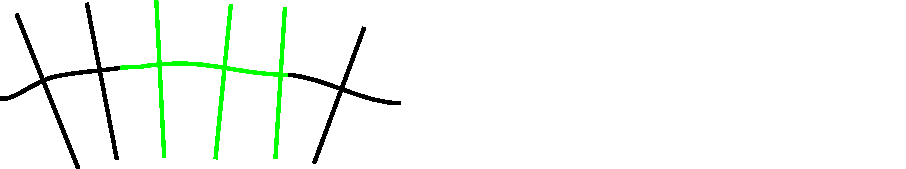
\includegraphics[width=8cm]{3_1 kart}
	\end{wrapfigure}

	Das heißt lokal lässt sich ein Bündel auffassen als karthesisches Produkt. Gibt es eine globale Trivialisierung (also $(\psi,U)$ Bündelkarte mit $U = B$), so heißt das Bündel \emph{trivial}.
\end{minipage}

\begin{exmp*}
	\begin{enumerate}[label = {\roman*})]
		\item 	Zylinder: $ \Sbb^1 \times \R \to \Sbb^1 $ ist trivial
			\image{3_1 zylinder}{2cm}
		\item "Unendlich ausgedehntes" Möbiusband  $ \pi: E \to \Sbb^1 $ von Rang 1, ein nicht triviales Bündel über $\Sbb^1$ mit Faser $\cong \R$ (später mehr)
			\image{3_1 moebius}{8cm}
		\item $ N = \{(p,v) \in \Sbb^2 \times \R^3 \mid v \| p\}\ (\Sbb^2 \subset \R^3) $
			\image{3_1 buendel}{12cm}
			Das Normalenbündel ist trivial.
		\item \begin{minipage}{\linewidth}
				\begin{wrapfigure}{R}{5cm}
					\centering
					
\includegraphics[width=5cm]{3_1 moebius2}
				\end{wrapfigure}
				(vgl. Diff 2)
			\end{minipage} \\
			$ M = $ Möbiusband\\
			$ \pi^{-1}(x) = \{\lambda n_x \mid \lambda \in \R\} $\\
			$ x \mapsto n_x$ Einheitsnormalen-Vektorfeld\\
			Das Bündel ist nicht trivial. (später mehr)
	\end{enumerate}
\end{exmp*}

\begin{defn}[Schnitt]\index{Vektorraumbündel!Schnitt}
	Ein \emph{Schnitt} eines Vektorraumbündels $ (E,\pi,B) $ ist eine stetige Abbildung $ z: B \to E $ mit $z(x) \in E_x\ \foralll x \in B$.
	\image{3_2}{8cm}
\end{defn}
	
\begin{exmp*}
	Nullschnitt: $ B \to E,\ x \mapsto 0 \in E_x $
	\image{3_2 nullschnitt}{12cm}
\end{exmp*}

\begin{rem*}
	$ z: B \to E $ Schnitt $ \implies z: B \to z(B) $ Homöomorphismus.\\
	$z_0$ Nullschnitt: $z_0(B) \cong B$.
\end{rem*}

\begin{defn}[Bündelatlas, Übergangsfunktion]\index{Vektorraumbündel!Bündelatlas} \index{Vektorraumbündel!Übergangsfunktion}
	Sei $ (E,\pi,B) $ ein Vektorraumbündel von Rang $n$. Eine Menge von Bündelkarten $ \{(\varphi_\alpha, U_\alpha) \mid \alpha \in A\} $ heißt \emph{Bündelatlas} von $E$, wenn $ \bigcup_{\alpha \in A} U_\alpha = B. $
	Die auf Überlappungen $ U_\alpha \cap U_\beta $ gegebenen stetigen Abbildungen 
	$$ \Phi_{\alpha \beta}: U_\alpha \cap U_\beta \to GL(n,\R),\ x \mapsto \bound{\varphi_\beta}{E_x} \circ \left( \bound{\varphi_\alpha}{E_x} \right)^{-1} $$
	heißen \emph{Übergangsfunktionen}.
\end{defn}

\begin{rem*}
	$\Phi_{\alpha \beta}$ nehmen tatsächlich Werte in $GL(n,\R)$ an:
	\image{3_3}{12cm}
	$$ \bound{\varphi_\beta}{E_x} \circ \left( \bound{\varphi_\alpha}{E_x} \right)^{-1}: \underset{\cong \R^n}{\{x \times \R^n\}} \to \underset{\cong \R^n}{\{x \times \R^n\}} $$
	ist ein Vektorraumisomorphismus für jedes $x$. (nach Definition Bündelkarte)
\end{rem*}

\begin{rem*}
	Es gilt die sogenannte \emph{Kozykelbedingung}:
	\image{3_3 kozykel}{14cm}
\end{rem*}

\begin{exmp*}
	$ \Sbb^1 \subset \R^2 $\\
	\begin{minipage}{\linewidth}
		\begin{wrapfigure}{R}{4cm}
			\centering
			
\includegraphics[width=4cm]{3_3 circ}
		\end{wrapfigure}
		$ U_1 = \Sbb^1 \setminus \{p_1\},\ U_2 = \Sbb^1 \setminus \{p_2\} $ (offen in $\Sbb^1$)\\
		überdeckt $\Sbb^1$: $ U_1 \cap U_2 = \left\{ \underset{V_+}{\bigcap}, \overset{V_-}{\bigcup} \right\} $\\
		Sind die Übergangsfunktionen $ \Phi_{21}(p) = \id_\R\ \foralll p \in U_1 \cap U_2 $, so ist das Bündel trivial. Denn dann kann man eine lokale Trivialisierung auf $ U \subset \Sbb^1 $ auf ganz $\Sbb^1$ fortsetzen. Man erhält den Zylinder.\\
		Wählen wir als Übergangsfunktion
		\begin{alignat*}{2}
			\Phi_{21}(p) &= \id_\R \qquad &&\foralll p \in V_+\\
			\Phi_{12}(p) &= -\id_\R \qquad &&\foralll p \in V_-
		\end{alignat*}
		erhält man das "Möbiusband" (unendlich ausgedehnt)
	\end{minipage}
	\image{3_3 geom}{15cm}
\end{exmp*}

\begin{defn*}
	Wie bei Mannigfaltigkeiten gilt: Ein Bündelatlas über einer differenzierbaren Mannigfaltigkeit heißt \emph{differenzierbar}, falls alle Übergangsfunktionen (als Funktionen von $p \in M = B$) glatt sind. Ein differenzierbares Vektorbündel ist ein Vektorbündel über $M$ mit einem maximalen differenzierbaren Bündelatlas.\\
	Eine Funktion $ f: E \to \tilde{E}\ (E,\tilde{E}$ differenzierbare Bündel) heißt differenzierbar/glatt in $p \in \pi(E)$, wenn $ \tilde{\varphi} \circ f \circ \varphi^{-1} $ differenzierbar/glatt in $\varphi(p)$ ist, wobei $(\varphi,U)$ eine Bündelkarte bei $p$ ist und $(\tilde{\varphi},\tilde{U})$ eine Bündelkarte bei $f(p)$ ist (jeweils aus dem maximalen differenzierbaren Bündelatlas). 
\end{defn*}

\begin{defn}[Prä-Vektorraumbündel, Prä-Bündelatlas] \index{Vektorraumbündel!Prä-Vektorraumbündel} \index{Vektorraumbündel!Prä-Bündelatlas}
	Ein \emph{Prä-Vektorraumbündel} ist ein Quadrupel $ (E,\pi,B,\Acal) $, wobei $E$ eine Menge ist, $B$ ein topologischer Raum, $\pi: E \to B$ surjektiv, sodass $E_x = \pi^{-1}(x)$ ein Vektorraum ist, und mit einem \emph{Prä-Bündelatlas} $\Acal$, das heißt einer Menge $ \{(\varphi_\alpha,U_\alpha) \mid \alpha \in A\} $, sodass $U_\alpha \subset B$ offen, $ B = \bigcup_{\alpha \in A} U_\alpha $ und $ \varphi_\alpha: \pi^{-1}(U) \to U \times \R^n $ bijektiv für alle $\alpha$, sodass $ \bound{\varphi_\alpha}{E_y}: E_y \to \{y\} \times \R^n $ ein Vektorraum-Isomorphismus ist und so, dass die Übergangsfunktionen 
	$ \begin{aligned}[t]
		\Phi_{\alpha \beta}: &U_\alpha \cap U_\beta \to GL(n,\R),\\
		 &x \mapsto \bound{\varphi_\beta}{E_x} \circ \left( \bound{\varphi_\alpha}{E_x} \right)^{-1}
	\end{aligned} $ stetig sind.
\end{defn}

\begin{rem}
	\begin{enumerate}[label= {\roman*})]
		\item Sei ein Prä-Vektorraumbündel $ (E,\pi,B,\Acal) $ gegeben. Wie in Lemma \ref{1.14} zeigt man, dass eine Topologie auf $E$ (eindeutig!) dadurch festgelegt ist, dass man fordert, dass $(E,\pi,B)$ ein Vektorraumbündel ist und $\Acal$ ein Bündelatlas. (Man erklärt die Topologie so, dass die $\varphi_\alpha$ Homöomorphismen sind.)
		\item Ist $M$ eine differenzierbare Mannigfaltigkeit und $ (E,\pi,M,\Acal) $ ein differenzierbares Prä-Vektorraumbündel (das heißt alle Übergangsfunktionen sind glatt) erhält man auf diese Art sogar ein differenzierbares Vektorraumbündel (die differenzierbare Struktur ist eindeutig durch $\Acal$ festgelegt durch Übergang zu $\Dcal(\Acal)$).
	\end{enumerate}
\end{rem}

\begin{exmp}
	Sei $M$ eine differenzierbare $n$-dimensionale Mannigfaltigkeit. Sei $\Acal$ ein differenzierbarer Atlas von $M$. Dann ist $(TM, \pi, M, \Acal)$ mit
	\begin{align*}
		TM &= \bigcup_{p \in M} T_pM\\
		\pi&: TM \to M,\quad T_pM \mapsto p\\
		\Acal&= \left\{ \begin{aligned}
			\varphi: \pi^{-1}(U) &\to U\times \R^n,\\
			 T_pM \ni X_p &\mapsto \left( p, X_p(\overbar{\varphi_1}), \dotsc, X_p(\overbar{\varphi_n}) \right)
		\end{aligned} \ \middle|\ (\varphi,U) \in \Acal \right\},
	\end{align*}
	wobei $ X_p (\overbar{\varphi_j}) = j $-te Koordinate von $X_p \in T_pM$ bezüglich $(\varphi,U)$ (vgl. Lemma \ref{2.7}),\\
	ein Prä-Vektorraumbündel.\\
	Das zugehörige differenzierbare Vektorraumbündel $TM$ über $M$ heißt das \emph{Tangentialbündel}. 
\end{exmp}

\begin{exmp*}
	$ T\Sbb^1 = \{(x,v) \in \Sbb^1 \times \R^2 \subset \R^4 \mid x \bot v\} $\\
	\begin{minipage}{\linewidth}
		\begin{wrapfigure}{R}{4cm}
			\centering
			
\includegraphics[width=4cm]{3_6}
		\end{wrapfigure}
		$ \pi: T\Sbb^1 \to \Sbb^1,\ \pi(x,v) = x $\\
		globale Trivialisierung: $ T\Sbb^1 \to \Sbb^1 \times \R,\ (x,v) \mapsto (x,\lambda) $, wobei $\lambda v = \begin{pmatrix}
			-x_2\\x_1
		\end{pmatrix}$\\
		Das Bündel ist also trivial.
	\end{minipage}
\end{exmp*}

\begin{rem*}
	$ \varphi_2^+ : U_2^+ \cap \Sbb^1 \to \R,\ \varphi_2^+(x_1,x_2) = x_1 $
	\begin{align*}
		X_{\gamma,x}\left( \overbar{\varphi_2^+} \right) &= \frac{d}{dt} \left( \overbar{\varphi_2^+} \circ \overbar{\gamma} \right) (0)\ \text{mit} \begin{aligned}[t]
			&\gamma: (-\epsilon,\epsilon) \to \Sbb^1\\
			&\gamma(0) = x\\
			&\gamma(t) = (\cos(t+\alpha),\sin(t+\alpha))
		\end{aligned}\\
		&= \begin{pmatrix}
			-\sin(\alpha) \\ \cos(\alpha)
		\end{pmatrix}
	\end{align*}
	Bündelkarte: $\varphi_{2,+}: \pi^{-1}(U_2^+ \cap \Sbb^1) \to U_2^+ \cap \Sbb^1 \times \R,\ \varphi_{2,+}(\underbrace{X_{p,x}}_{\in Tx\Sbb^1}) = \left( x, X_{\gamma,x}\left( \overbar{\varphi_2^+} \right) \right)$\\
	Für die anderen Koordinatenbereiche sieht die Karte ebenso aus.
	$$ \varphi_{j,\pm} (\underbrace{\lambda X_{p,x}}_{\in T_xM}) = \left( \begin{pmatrix}
		\cos(\alpha)\\\sin(\alpha)
	\end{pmatrix}, \lambda \begin{pmatrix}
	-\sin(\alpha)\\\cos(\alpha)
	\end{pmatrix} \right) $$
	Übergangsfunktionen: $\id_\R$
\end{rem*}

\begin{defn}[Vektorfeld] \index{Mannigfaltigkeit!Vektorfeld}
 	Ist $M$ eine differenzierbare Mannigfaltigkeit, so nennt man einen differenzierbaren Schnitt $z: M \to TM$ ein \emph{Vektorfeld} auf $M$.
\end{defn}

\begin{rem*}
	Das Tangentialbündel ist als Vektorbündel eine Mannigfaltigkeit. Dann ist ein glatter bzw. differenzierbarer Schnitt $z: M \to TM$ eine glatte Abbildung zwischen Mannigfaltigkeiten, sodass $\pi \circ z$ die Identität ist.
\end{rem*}

\begin{defn}[Differential]\index{Differential}
	Ist $ f: M \to N $ glatt, so ist durch $ T_pf: T_pM \to T_{f(p)}N $ eine differenzierbare Abbildung
	\[ Tf: TM \to TN \] gegeben. $Tf$ nennt man das \emph{Differential}.
	\image{3_8}{14cm}
\end{defn}
	\section{Konstruktionen mit Vektorbündeln}

\begin{rem}\lecture
	Die folgenden Konstruktionen werden für topologische Vektorbündel formuliert, gelten jedoch \emph{mutatis mutandis} (dies ändert, was zu ändern ist) auch für differenzierbare Vektorbündel (ersetze "stetig" durch "glatt" etc.)
\end{rem}

\begin{defn}[Bündel-Homomorphismus]\index{Vektorraumbündel!Bündel-Homomorphismus}\label{3.10}
	Seien $ (E,\pi,B),(\tilde{E},\tilde{\pi},\tilde{B}) $ Vektorraumbündel. Ein \emph{Bündel-Homomorphismus} ist ein Paar von stetigen Abbildungen $f: E \to \tilde{E}$ und $g: B \to \tilde{B}$, sodass
	\[ \begin{tikzcd}
		E \arrow{r}{f} \arrow{d}{\pi} & \tilde{E} \arrow{d}{\tilde{\pi}}\\
		B \arrow{r}{g} & \tilde{B}
	\end{tikzcd} \]
	kommutiert, also $g \circ \pi = \tilde{\pi} \circ f$, und $ f_x := \bound{f}{E_x}: E_x \to \tilde{E}_{g(x)} $ linear ist für alle $x \in B$.
\end{defn}

Sind $f$ und $g$ wie oben sogar Homöomorphismen und $f_x$ ein Vektorraum-Isomorphismus, so liegt ein \emph{Vektorbündel-Isomorphismus} vor.

\begin{exmp*}
	Der Isomorphismus $ T\Sbb^1 \cong \Sbb^1\times \R $ ist ein Vektorbündel-Isomorphismus.
\end{exmp*}

\begin{defn}[Unterbündel]\index{Vektorraumbündel!Unterbündel}
	Ist $ (E,\pi,B) $ ein Vektorbündel von Rang $n$ und $\tilde{E} \subset E$ eine Teilmenge, sodass es um jedes $x \in B$ eine Bündelkarte $(\varphi,U)$ gibt, sodass
	\[ \varphi \left(\pi^{-1}(U) \cap \tilde{E} \right) = U \times \R^k \subset U \times \R^n, \]
	so ist $ \left( \tilde{E}, \bound{\pi}{\tilde{E}},B \right) $ ein Vektorbündel von Rang $k$, ein sogenanntes \emph{Unterbündel}.
\end{defn}

\begin{lem}
	Sei $f: E \to \tilde{E}$ ein Bündel-Homomorphismus von Vektorbündeln über $B$ ($g = \id_B$ in Definition \ref{3.10}). Sei der Rang $f_x = m$ konstant für alle $x \in B$. Dann ist
	\begin{itemize}
		\item $ \ker f := \bigcup_{x \in B} \ker f_x $ ein Unterbündel von $E$ von Rang $n-m$ ($n = $ Rang von $E$),
		\item $ \im f := \bigcup_{x \in B} \im f_x $ ein Unterbündel von $\tilde{E}$ von Rang $m$.
	\end{itemize}
	\image{3_12}{14cm}
\end{lem}

\begin{defn}[Einschränkungen]\index{Vektorraumbündel!Einschränkungen}
	Ist $ (E,\pi,B) $ ein Vektorbündel und $\tilde{B} \subset B$ eine Teilmenge, so ist
	\[ \left( \pi^{-1} \left( \tilde{B} \right), \bound{\pi}{\pi^{-1} \left( \tilde{B} \right)}, \tilde{B} \right) \]
	ein Vektorbündel ("Einschränkung von $E$ auf $\tilde{B}$").
	\image{3_13}{8cm}
\end{defn}

\begin{defn}[Pullback-Bündel]\index{Vektorraumbündel!Pullback-Bündel}
	Sei $ (E ,\pi,B) $ ein Vektorbündel über $B$ und $f: B_0 \to B$ stetig. Dann ist durch
	\[ f^*E := \{(x,e) \in B_0 \times E \mid f(x) = \underbrace{\pi(e)}_{\in B}\} \subset B_0 \times E \]
	ein Bündel über $B_0$ erklärt mit $ \pi_0(x,e) = x, $ das \emph{von $f$ induzierte Bündel} bzw. das \emph{Pullback-Bündel entlang $f$}.
	\image{3_14}{14cm}
\end{defn}

\begin{rem}
	Die Konstruktion ist so gewählt, dass wenn $\pi_2: f^*E \to E$ die Projektion auf den 2. Faktor bezeichnet, das Diagramm
	\[ \begin{tikzcd}
		f^*E \arrow{r}{\pi_2} \arrow{d}{\pi_0} & E \arrow{d}{\pi}\\
		B_0 \arrow{r}{f} & B
	\end{tikzcd} \]
	kommutiert.\\
	Lokale Trivialisierung: Sei $ (\varphi,U) $ eine Trivialisierung von $E$ bei $f(x)$. Dann ist $ (\psi,f^{-1}(U)) $ eine lokale Trivialisierung von $f^*E$ bei $x$, wobei $ \psi(y,e) = (y,\pi_2(\underbrace{\varphi(e)}_{\in U \times \R^n})). $
\end{rem}

\begin{defn}[Lineare Abbildung, Bündelabbildung]\index{Vektorraumbündel!lineare Abbildung}\index{Vektorraumbündel!Bündelabbildung}
	Seien $ (E,\pi,B) $ und $ (\tilde{E},\tilde{\pi}\tilde{B}) $ Vektorbündel über $B$ bzw. $\tilde{B}$. Sei $f: B \to \tilde{B}$ stetig. Dann heißt eine stetige Abbildung $\tilde{f}: E \to \tilde{E}$ \emph{lineare Abbildung über $f$}, falls $ \bound{\tilde{f}}{E_x}: E_x \to \tilde{E}_{f(x)} $ linear ist für alle $x \in B$. Sind alle $ \bound{\tilde{f}}{E_x} $ Vektorraum-Isomorphismen, so heißt $\tilde{f}$ \emph{Bündelabbildung über $f$}.
\end{defn}
	
\begin{exmp*}
	\[ \begin{aligned}
		\tilde{f}:& f^*E \to E\\
		\tilde{f}:& B_0 \times E \to E
	\end{aligned},\ f:B_0 \to B \ \text{stetig} \]
	ist eine Bündelabbildung über $f$. ("kanonische Bündelabbildung")
\end{exmp*}

\begin{lem}
	Ist $ g: E \to \tilde{E} $ eine lineare Abbildung von Vektorbündeln $(E,\pi,B), (\tilde{E}, \tilde{\pi},\tilde{B})$ über $f: B \to \tilde{B}$, so gibt es einen eindeutigen Bündel-Homomorphismus $h: E \to f^*\tilde{E}$, sodass $g = \tilde{f} \circ h$ ist, wobei $ \tilde{f}: f^*\tilde{E} \to \tilde{E} $ die kanonische Bündelabbildung ist:
	\[ \begin{tikzcd}
		E \arrow{r}{\exists !h} \arrow{dr}{\pi} \arrow[bend left=35]{rr}{g} & f^*\tilde{E} \arrow{r}{\tilde{f}} \arrow{d}{\pi_1} & \tilde{E} \arrow{d}{\tilde{\pi}} \\
			& B\arrow{r}{f} & \tilde{B}
		\end{tikzcd} \]
\end{lem}

\begin{exmp*}
	Die Differentiale $ T_pf: T_pM \to T_{f(p)}N $, für $f:M \to N$ glatt, definieren das Differential $Tf: TM \to TN$. Es gibt genau einen Bündel-Homomorphismus $h: TM \to f^TN$, sodass
	\[ \begin{tikzcd}
		TM \arrow{rr}{Tf} \arrow{dr}{h}&&TN\\
		& f^*TN \arrow{ur}{\tilde{f}}
	\end{tikzcd} \qquad \text{kommutiert.} \]
\end{exmp*}
	\lecture Faserweise kann man nun Konstruktionen der linearen Algebra vornehmen: direkte Summe, Tensorprodukt, Dualraum etc.

\begin{exmp}\label{3.18}
	\begin{enumerate}[label={\roman*})]
		\item Direkte Summe:\\
			Seien $ (E,\pi,B),(\tilde{E},\tilde{\pi},B) $ Vektorbündel über $B$. Dann ist die \emph{direkte Summe}
			\[ E \oplus \tilde{E} := \bigcup_{x \in B} E_x \oplus \tilde{E}_x \]
			auch wieder ein Vektorbündel (von Rang $n + \tilde{n}$)
		\item Tensorprodukt:
			\[ E \otimes \tilde{E} := \bigcup_{x \in B} E_x \otimes \tilde{E}_x \]
		Bündel-Atlas:
			\begin{gather*}
				\big\{ (\varphi \otimes \psi, U \cap V) \mid (\varphi,U) \in \text{Atlas von }E,\ (\psi,V) \in \text{Atlas von } \tilde{E} \big\}\\
				\bound{\varphi \otimes \psi}{E_x \otimes \tilde{E}_x} : E_x \times \tilde{E}_x \to \{x\} \times \R^n \otimes \R^{\tilde{n}}
			\end{gather*}
		\item Duales Bündel: $ E^* = \bigcup_{x \in B} E_x^* $\\
			$ \pi_{E^*} $ so, dass $ \pi_{E^*}^{-1} (x) = E_x^* = \Hom(E_x,\R) $\\
			Bündelatlas: Ist $ (\psi,U) \in $ Atlas von $E$, so ist 
			$$ \psi^*: \pi_{E^*}^{-1} (U) \to U \times \R^n,\ E_x^* \ni \alpha_x \mapsto (x,w),$$
				wobei $w$ der eindeutige Vektor $\in \R^n$ ist, sodass
			\[ \alpha_x (v_x) = \langle w,pr_2(\underbrace{\psi(v_x)}_{\in \{x\} \times \R^n}) \rangle \quad \foralll v_x  \in E_x \]
	\end{enumerate}
\end{exmp}

Speziell für das Tangentialbündel:

\begin{defn}[Kotangentialbündel]\index{Vektorraumbündel!Kotangentialbündel}
	Das \emph{Kotangentialbündel} $T^*M$ an einer differenzierbaren Mannigfaltigkeit $M$ ist das zu $TM$ duale Bündel. $ (T_pM)^* =: T_p^*M $ heißt \emph{Kotangentialraum}.
\end{defn}

In Koordinaten: Seien $ (x_1,\dotsc,x_n) $ lokale Koordinaten bei $p \in M$, $ \big( \bound{\del{x_1}}{p},\dotsc, \bound{\del{x_n}}{p} \big) $ eine Basis von $T_pM$. Hierbei betrachten wir nicht unbedingt bei $p$ zentrierte Karten $ (\varphi,U) $ von $M$.\\
Es ist dann für $f \in C^\infty(U)$ beziehungsweise Keim bei $p$
\begin{align*}
	\bound{\del{x_j}}{p}f &= \bound{\del{x_j}}{\varphi(p)} (f \circ \varphi^{-1})\\
	&= \del{x_j} \hat{f} (\hat{p}),
\end{align*}
mit $\hat{p} = \varphi(p)$ und $\hat{f} = f \circ \varphi^{-1}$ als Koordinatendarstellung von $f$.

\begin{rem}
	Kartenwechsel
	\incfig{3_20}{8cm}
	Die Tangentialabbildung $T_p\Phi$ bezüglich der Basen $ (\del{x_1},\dotsc, \del{x_n}),(\del{y_1},\dotsc,\del{y_n}) $ ist die Jacobimatrix $ \begin{pmatrix}
		\del{x_1} \Phi_1 & \cdots & \del{x_n}\Phi_1\\
		\vdots & &\vdots\\
		\del{x_1}\Phi_n & \cdots & \del{x_n}\Phi_n
	\end{pmatrix} = D\Phi, $ also $ T_p\Phi(\del{x_i}) = \sum \del{x_i}\Phi_j ({\vertarrowbox[3pt]{\hat{p}}{Koord. von $p$, also $\varphi(p)$}}) \del{y_j}. $
\end{rem}

Merke: $ \Phi_j(\hat{p}) = \psi_j(p) = y_j $\\
Man schreibt daher auch
\[ \bound{\del{x_i}}{p} = \sum_{j=1}^{n} \frac{\del{y_j}}{\del{x_i}}(p) \bound{\del{y_j}}{p} \]
Denn $T_p\Phi$ transponiert nicht in einen anderen Tangentialraum, sondern bildet wieder (sogar isomorph) nach $T_pM$ ab. (Basiswechsel!)\\
In der Notation unterscheiden wir $p$ und $\hat{p}$, $f$ und $\hat{f}$ meist nicht.

\begin{exmp}
	\begin{enumerate}[label={\roman*})]
		\item $ M = \R^2 $, kartesische vs. Polarkoordinaten\\
			$ \Phi = \psi \circ \varphi^{-1}, \varphi^{-1}(r,\theta) = \begin{pmatrix}
				r \cos \theta \\ r \sin \theta
			\end{pmatrix}, r \in \R_{\geq 0}, \theta \in (0,2\pi), \psi(x_1,x_2) = \begin{pmatrix}
			x_1\\x_2
			\end{pmatrix} $\\
			Betrachte $v \in T_p\R^2, v = \bound{\del{r}}{p} - \bound{\del{\theta}}{p},\ p = \begin{pmatrix}
				0\\2
			\end{pmatrix},\ (r=2,\theta = \frac{\pi}{2})$\\
			\begin{minipage}{\linewidth}
				\begin{wrapfigure}{R}{4cm}
					\centering
%					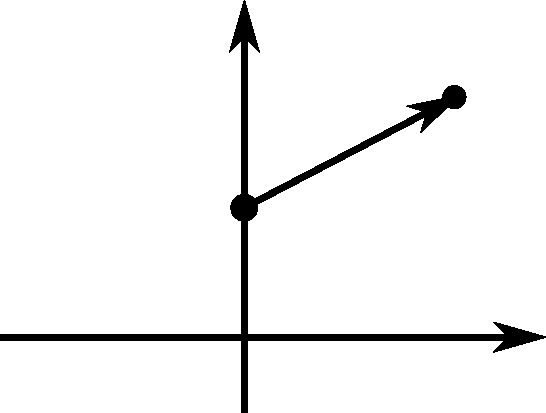
\includegraphics[width=4cm]{3_21 i}
					\wrapincfig{3_21 i}{4cm}
				\end{wrapfigure}
				
				$ \del{r} \Phi \big(2,\frac{\pi}{2} \big) = \begin{pmatrix}
					0\\1
				\end{pmatrix}, \quad \del{\theta} \Phi \big( 2,\frac{\pi}{2} \big) = \begin{pmatrix}
					-2\\0
				\end{pmatrix} $\\
				$ \implies \begin{aligned}[t]
					\bound{\del{r}}{p} &= 0 \cdot \bound{\del{x_1}}{p} + \bound{\del{x_2}}{p}\\
					\bound{\del{\theta}}{p} &= -2 \bound{\del{x_1}}{p}
				\end{aligned} $\\
				$ \implies v $ hat in kartesischen Koordinaten die Darstellung $ \bound{\del{x_2}}{p} + 2 \bound{\del{x_1}}{p} $
			\end{minipage}
		\item $ \Phi(x,y) = \begin{pmatrix}
			x\\p+x^3
			\end{pmatrix} = \begin{pmatrix}
				\tilde{x}\\\tilde{y}
			\end{pmatrix}, p = \begin{pmatrix}
				1\\0
			\end{pmatrix} $\\
			$ \bound{\del{x}}{p}\Phi = \begin{pmatrix}
				1\\3
			\end{pmatrix}, \bound{\del{y}}{p}\Phi = \begin{pmatrix}
				0\\1
			\end{pmatrix} $\\
			$ \implies \begin{aligned}[t]
				\bound{\del{x}}{p} &= \bound{\del{\tilde{x}}}{p} + 3\bound{\del{\tilde{y}}}{p} \neq \bound{\del{\tilde{x}}}{p} \ \text{obwohl } \tilde{x} = x\ \text{ist}\\
				\bound{\del{y}}{p} &= \bound{\del{\tilde{y}}}{p}
			\end{aligned}$
	\end{enumerate}
\end{exmp}

\begin{rem}\label{3.22}
	Beachte: Schreibt man ein Element $v \in T_pM$ als $ v = \sum v_i \bound{\del{x_i}}{p} = \sum \tilde{v}_j \bound{\del{y_j}}{p} $, so gilt also
	\[ \sum_{i=1}^{n} v_i \bound{\del{x_i}}{p} = \sum_{i=1}^{n} v_i \sum_{j=1}^n \frac{\del{\Phi_j}}{\del{x_i}}(\hat{p}) \bound{\del{y_j}}{p}, \]
	\[ \text{Also } \tilde{v}_j = \sum_{i=1}^n \del{x_i} \Phi_j(\hat{p}) v_i\quad \text{"kovariantes Transformationsverhalten"} \]
	Wie transformieren sich Elemente des Kotangentialraums? Sei $w \in T_pM^*$. Bezeichne $ (\bound{\alpha_1}{p},\dotsc, \bound{\alpha_n}{p}) $ die zu $ (\del{x_1},\dotsc, \del{x_n}) $ duale Basis, $ (\bound{\tilde{\alpha}_1}{p},\dotsc, \bound{\tilde{\alpha}_n}{p}) $ die zu $ (\del{y_1},\dotsc, \del{y_n}) $. Dann schreibt sich $w$ als 
	\[ w = \sum w_i \bound{\alpha_i}{p} = \sum \tilde{w}_j \bound{\tilde{\alpha}_j}{p}, \]
	wobei $w_i = w \big( \bound{\del{x_i}}{p} \big)$ und $\tilde{w}_j = w \Big( \bound{\del{y_j}}{p} \Big)$. Somit folgt
	\begin{align*}
		w_i &= w \big( \bound{\del{x_i}}{p} \big) = w \Bigg( \sum_{j=1}^n \underbrace{\del{x_i} \Phi_j(\hat{p})}_{\in \R} \bound{\del{y_j}}{p} \Bigg)\\
		&= \sum_{j=1}^n \del{x_i} \Phi_j(\hat{p}) \tilde{w}_j\quad \text{"kontravariantes Transformationsverhalten"}
	\end{align*}
	Beziehungsweise für die Basis:
	\[ \tilde{\alpha}_j = \sum_{i=1}^n \del{x_i}\Phi_j (\hat{p}) \bound{\alpha_i}{p} \]
\end{rem}
\addtocounter{thm}{1}
\begin{defn}[Differential-Eins-Form]\index{Differentialform}
	Ein glatter Schnitt $M \to T^*M$ heißt \emph{Differential-Eins-Form}. Die Menge der Differentialformen bezeichnet man mit $\Omega^1(M)$. Ist $U \subset M$ offen, so bezeichnet man die Menge der glatten Schnitte $ U \to \bound{T^*M}{U} $ mit $\Omega^1(U)$.
\end{defn}

In Koordinaten: Die Koeffizientenfunktion hängt glatt von $p \in M$ ab:

\begin{exmp*}
	$p \mapsto T_pf,\ f \in C^\infty(M)$, das Differential von $f$ ist $\in \Omega^1(M)$. Man schreibt dafür auch $df$ (anstelle von $p \mapsto T_pf$). Denn:\\
	In Koordinaten gilt $ T_pf \big( \bound{\del{x_i}}{p} \big) = \del{x_i} f(p) $ (denn $T_pf$ ist in dieser Basis die Jacobimatrix!), das heißt $\bound{df}{p}$ lässt sich schreiben als
	\[ \bound{df}{p} = \sum_{i=1}^n \del{x_i} f(p) \bound{\alpha_i}{p} \quad \leftarrow \text{duale Basis zu }\del{x_1},\dotsc, \del{x_n} \]
	Insbesondere gilt für die Koordinatenfunktion $ f = x_j: \bound{dx_j}{p} = \bound{\alpha_j}{p}. $\\
	Diese Notation wollen wir daher im Folgenden für die duale Basis verwenden.
\end{exmp*}

\begin{lem}
	Sei $ (\varphi,U) $ eine Karte von $M$ bei $p \in U$. Dann lässt sich jedes $ \alpha \in \Omega^1(M) $ schreiben als
	\[ \alpha = \sum_{i=1}^n f_i d x^i, \]
	$dx_i \in \Omega^1(U)$, mit $f_i \in C^\infty(U)$ eindeutig bestimmt.
\end{lem}

\begin{exmp*}
	$ \Phi(r,\theta) = \begin{pmatrix}
		r\cos\theta\\ r \sin\theta
	\end{pmatrix} $\\
	$\alpha \in \Omega^1(\R^2) \implies w = f(x,y)dx + g(x,y)dy$, $f$ und $g$ glatt.\\
	Wir könnten die Formel aus \ref{3.22} verwenden,
	\[ \bound{\tilde{\alpha}}{p} = \sum_{i=1}^n \del{x_i} \Phi_j (\hat{p}) \bound{\alpha_i}{p}, \]
	schneller geht es direkt:
	\begin{align*}
		dh &= \sum \del{y_j} h dy^i\\
		d(r\cos\varphi) &= \cos\varphi dr - r \sin\varphi d\varphi\\
		d(r\sin\varphi) &= \sin\varphi dr + r \cos\varphi d\varphi
	\end{align*}
	\begin{align*}
		\implies w &= \Big(f \big(r\cos\theta,r\sin\theta \big)\cos\theta + g \big(r\cos\theta,r\sin\theta \big)\sin\theta\Big) dr\\
		&+ r\Big(-f \big(r\cos\theta,r\sin\theta \big)\sin\theta + g \big(r\cos\theta,r\sin\theta \big)\cos\theta\Big) d\theta
	\end{align*} 
\end{exmp*}
	
	
	
	
	

	\printindex
\end{document}